\subsection{Problem}
\renewcommand{\theequation}{\theenumi}
\begin{enumerate}[label=\thesection.\arabic*.,ref=\thesection.\theenumi]
\numberwithin{equation}{enumi}
	\item Given that the two numbers appearing on throwing two dice are different. Find the probability of the event ’the sum of numbers on the dice is 4’.\\
	\solution  
	
When a dice is thrown the sample space = Total number of possibilities(S)
\begin{align}
\myvec{\bmat{1&1}&\bmat{1&2}&\bmat{1&3}&\bmat{1&4}&\bmat{1&5}&\bmat{1&6}\\
\bmat{2&1}&\bmat{2&2}&\bmat{2&3}&\bmat{2&4}&\bmat{2&5}&\bmat{2&6}
\\\bmat{3&1}&\bmat{3&2}&\bmat{3&3}&\bmat{3&4}&\bmat{3&5}&\bmat{3&6}
\\\bmat{4&1}&\bmat{4&2}&\bmat{4&3}&\bmat{4&4}&\bmat{4&5}&\bmat{4&6}
\\\bmat{5&1}&\bmat{5&2}&\bmat{5&3}&\bmat{5&4}&\bmat{5&5}&\bmat{5&6}
\\\bmat{6&1}&\bmat{6&2}&\bmat{6&3}&\bmat{6&4}&\bmat{6&5}&\bmat{6&6}}
\end{align}
We need to find the probability that the sum of the numbers on the dice is 4, given that the two numbers are different


Let F denote the event 'numbers are different' and E denote the event 'sum of the numbers is 4'. We need to find $P\brak{\frac{E}{F}}$.\\
	
	The possibilities satisfying event E are 	
\begin{align}
	\myvec{\bmat{1&3}&\bmat{3&1}&\bmat{2&2}}
\end{align}
\begin{align}
	P\brak{E} = \frac{3}{36} = \frac{1}{12}
\end{align}
	
	The possibilities satisfying event F are 	
\begin{align}
\myvec{\bmat{1&2}&\bmat{1&3}&\bmat{1&4}&\bmat{1&5}&\bmat{1&6}\\
\bmat{2&1}&\bmat{2&3}&\bmat{2&4}&\bmat{2&5}&\bmat{2&6}
\\\bmat{3&1}&\bmat{3&2}&\bmat{3&4}&\bmat{3&5}&\bmat{3&6}
\\\bmat{4&1}&\bmat{4&2}&\bmat{4&3}&\bmat{4&5}&\bmat{4&6}
\\\bmat{5&1}&\bmat{5&2}&\bmat{5&3}&\bmat{5&4}&\bmat{5&6}
\\\bmat{6&1}&\bmat{6&2}&\bmat{6&3}&\bmat{6&4}&\bmat{6&5}}
\end{align}
\begin{align}
	P\brak{F} &= \frac{30}{36} = \frac{5}{6}\\	
	Also E\cap F &= \myvec{\bmat{1&3}&\bmat{3&1}}\\
	P\brak{E\cap F} &= \frac{2}{36} = \frac{1}{18}\\
	P\brak{\frac{E}{F}} &= \frac{P\brak{E\cap F}}{P\brak{F}}\\
	P\brak{\frac{E}{F}} &= \frac{\frac{2}{36}}{\frac{2}{30}} = \frac{1}{15}
\end{align}
	










	\begin{comment}
	\begin{figure}[!ht]
	\centering
	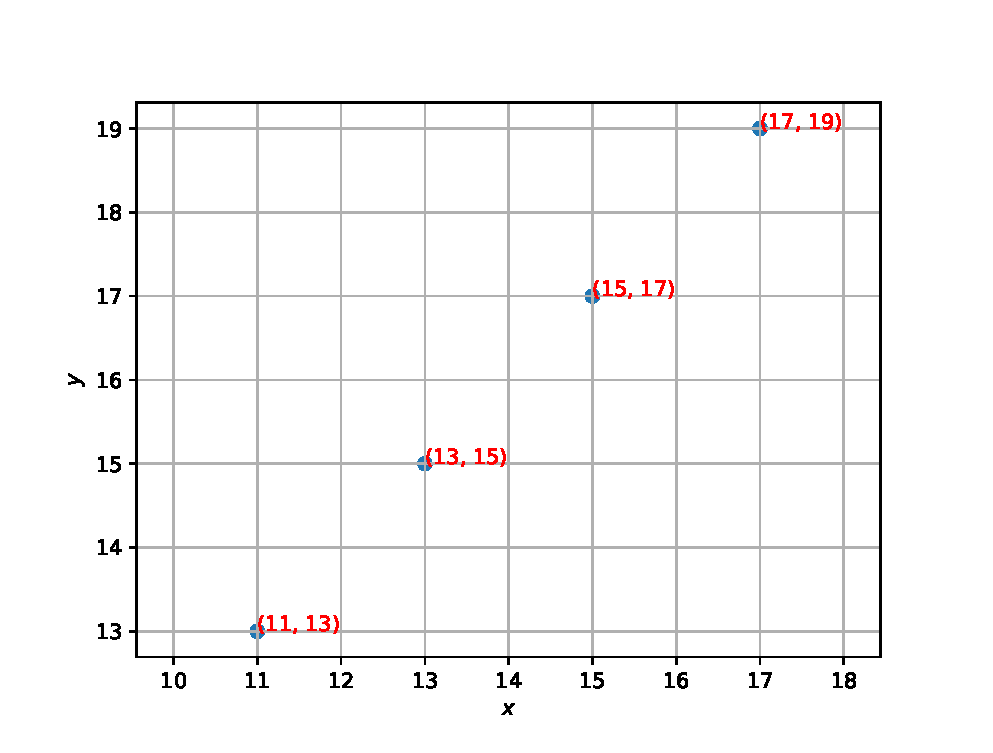
\includegraphics[width=\columnwidth]{./figs/lines/q15.eps}
	\caption{Triangle of Q.3.11.5}
	\label{fig:qfifteen}	
	\end{figure}
	\end{comment}	
	
\end{enumerate}
